
\chapter{Literature review}

\section{Economic Background}
\subsection{Labour (Employment) Demand \& Dynamics}

Labour demand is defined as the number of people that employers are willing to employ at a given wage during a specific time period~\textcolor{red}{\cite{TODO}}.

As a result of various economic phenomena, Labour demand is dynamic and frequently changes:
Firm-level performance, competition and policies in minimum-wage or taxation are among the many factors that can influence a firm's capacity to employ.
At the microeconomic (firm/individual) scale, much of the negative effects of labour demand equilibria changes Are expected in a free-market economy.

There are, however, systematic shocks that would affect the labour demand on a macroeconomic (economy-wide) sense. These can be deeply damaging to the proper functioning of that economy.
Examples of such systematic shocks include war, pandemics or financial crises.
Broadly, these shocks will have effects that extend to beyond labour demand shifts, since the economy is composed of an unfathomably complex network of cause-effect relationships.

Such a consequence of this interconnectedness is the existence of feedback loops within the economy, as the standard Keynesian representation of recessions depicts~\cite{mankiw2000macroeconomics} (see Figure~\ref{fig:recession-loop}):


\begin{figure}[ht]
    \caption{The inter-connected Economy}
    \label{fig:recession-loop}
    \centering
    \begin{minipage}{0.45\textwidth}
        \centering
        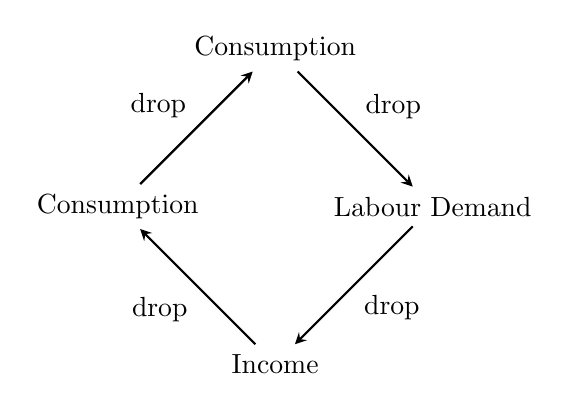
\begin{tikzpicture}[node distance=3cm, ->, >=stealth, thick]
            % Nodes placed in a circle
            \node (Consumption) at (0,2) {Consumption};
            \node (Labour Demand) at (2,0) {Labour Demand};
            \node (Income) at (0,-2) {Income};
            \node (back) at (-2,0) {Consumption};

            % Arrows with "drop" labels
            \draw[->] (Consumption) -- (Labour Demand) node[midway, above right] {drop};
            \draw[->] (Labour Demand) -- (Income) node[midway, below right] {drop};
            \draw[->] (Income) -- (back) node[midway, below left] {drop};
            \draw[->] (back) -- (Consumption) node[midway, above left] {drop};
        \end{tikzpicture}
        \caption*{Recession Cycle (Negative Feedback)}
    \end{minipage}
    \hfill
    \begin{minipage}{0.45\textwidth}
        \centering
        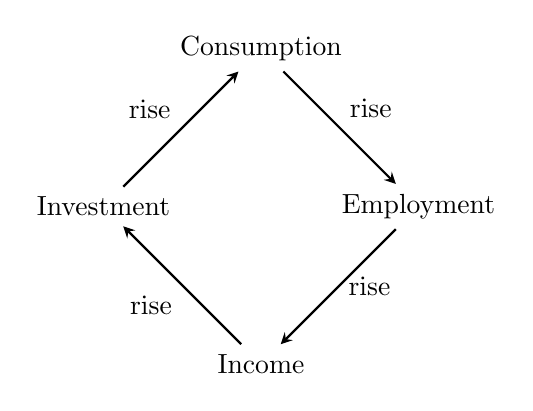
\begin{tikzpicture}[node distance=3cm, ->, >=stealth, thick]
            % Positive (recovery) cycle
            \node (consumption) at (0,2) {Consumption};
            \node (employment) at (2,0) {Employment};
            \node (investment) at (-2,0) {Investment};
            \node (income) at (0,-2) {Income};

            % Arrows with "rise" labels
            \draw[->] (consumption) -- (employment) node[midway, above right] {rise};
            \draw[->] (employment) -- (income) node[midway, right] {rise};
            \draw[->] (income) -- (investment) node[midway, below left] {rise};
            \draw[->] (investment) -- (consumption) node[midway, above left] {rise};
        \end{tikzpicture}
        \caption*{Recovery Cycle (Positive Feedback)}
    \end{minipage}
\end{figure}

\subsection{Theories of Innovation}

Another driver of shifts in Labour demand is technology, or more generally, as innovation. Classical economic theory and some research suggests that technological development \& adoption can be seen as a labour augmentation device, contributing positively to long term growth and employment~\cite{mankiw2000macroeconomics,ross_2024_LabourMarket}.
An opposing view, most famously represented by the example of the Luddites \cite{_2025_LudditeIndustrial}, depicts technological advancement as detrimental to employment prospects.

The theories of innovation are a historically rich field of research. One guiding theory is the \emph{Combinatorial view of Innovation}, originally envisioned by Schumpeter \cite{croitoru_2017_SchumpeterJoseph}.
This is the view that much of innovation derives from combining aspects of existing knowledge in novel ways, and it is empirically justified in a wide variety of scenarios.

For example, the widely cited work \cite{uzzi_2013_AtypicalCombinations} examines the nature of innovative research papers, and finds ``The highest-impact science is primarily grounded in exceptionally conventional combinations of prior work yet simultaneously features an intrusion of unusual combinations''.

Rogers' (1983) \emph{Diffusion of Innovations} is another theory of innovation focuses on the factors that determine how diffusive an innovation is - diffusion in this case is the ``process by which an innovation is communicated through certain channels over a period of time among members of a particular culture'' \cite{rogers_1983_DiffusionInnovations}.
Rogers depicts that there are four elements affecting the spread of new ideas, which model the transition as resulting from social and network factors. The wide-adoption of an innovation is integral to its sustenance on this view, but its key insight is that social networks hold the key to understanding whether an innovation will prevail.

There are many other theories of innovation. The authors of~\cite{wei_2023_MetaTheories} assess and classify the meta-theories of technological innovation from classical texts and modern sources.
Among their findings is that there are a wide variety of views on the dynamics of technological innovation, each exhibiting different causal understandings as depicted by the authors' meta-theory classifications.

\subsection{Role of Artificial Intelligence}

Artificial intelligence is perhaps in a separate category of technological innovation for a few reasons.
As is its nature, it is a different type of technology as it is inherently regarded as \emph{intelligence}. This can be seen as both complementary and substitutional to human intelligence or labour~\textcolor{red}{\cite{TODO}}.

This gives rise to emergent phenomena as it relates to technological innovation and labour:
\begin{enumerate}
  \item \textbf{AI \emph{as} innovation}: AI as a technology in the classical efficiency multiplier sense.
  \item \textbf{AI \emph{drives} innovation}:The authors of~\cite{liu_2020_InfluenceArtificial} examine the effects that AI has \emph{on other} technological innovation, finding a strong positive relationship, especially in low-tech sectors.
  \item \textbf{AI \emph{replaces} innovation}: Artificial General Intelligence (AGI) is the abstract concept of a technology with an intelligence surpassing that of all humanity~\textcolor{red}{\cite{TODO}}.
\end{enumerate}

It is the 3rd point here that is of deep importance, because it represents such a profound shift a civilizational sense.
Aside from the controversy and disagreement that surrounds the topic of AGI~\textcolor{red}{\cite{TODO}}, it is clear that Labour demand will be profoundly impacted by the continual development of AI~\textcolor{red}{\cite{TODO}}.


\section{Labour Demand Forecasting}
\subsection{Overview}

The practice of forecasting the demand (and \emph{supply}) for labour has a long history~\textcolor{red}{\cite{TODO}}.
Many critique its utility~\cite{thomas_2015_ReviewBest}, but there is good reason to believe that the limitations faced by current approaches are not insurmountable.
What follows is the findings of research into existing approaches, with an emphasis on their limitations.
\subsection{Typological Approaches to Forecasting}

\subsubsection{Manpower Requirements Approach~\cite{thomas_2015_ReviewBest}}
The authors of~\cite{thomas_2015_ReviewBest} discuss the \emph{Manpower Requirements Approach (MRA)} for forecasting labour demand, within the context of Aboriginal Canadian communities.
For context, the MRA approach is still central to the US's Bureau of Labour Statistics (BLS) occupational-forecasting methodology, among other major institutions.
In summary, the approach utilizes a ``future macroeconomic reference scenario for GDP [...] to derive an estimate of total employment demand, which is later broken down by industry and by occupation.''

The authors modify the approach slightly, due to some concerns about feasibly producing ``macroeconomic reference'' scenarios as they concern the Aboriginal population of Canada.
As a result, alongside a separate model they define for labour supply, their methodology is considered to be a fairly comprehensive framework for understanding demand \& supply.

An important contribution they make is to lament the importance of forecasting not only ``Expansion'' demand (an increase in demand in absolute terms) but also \emph{``Replacement''} demand (an increase in demand resulting from gaps created by mortality, retirements, occupational mobility, etc.).

However, the methodology is deeply assumption-led and is consequently limited.
\begin{itemize}
  \item \textbf{Static occupational coefficients:} They assume that occupational distribution by industry remains constant over time
  \item \textbf{Zero elasticity of substitution between labour types:}  workers in different occupations aren't easily substitutable.
  \item \textbf{Extrapolation of trends:} e.g., labour force participation or enrolment rates follow past patterns—even if future social or structural shifts may alter them significantly.
\end{itemize}

Furthermore, as the authors recognize, the framework is fraught with other issues including:
\begin{itemize}
  \item Data Limitation problems for smaller institutions
  \item An assumed heterogeneity of individuals within occupations misses a granular understanding of the individuals' differences (e.g. their skill-sets)
\end{itemize}

To add to data limitation problems, the authors find that a best practice is to use ``up-to-date data and regularly refresh forecasts (every 2–3 years, medium-term horizon of 5–10 years)''.
This is insufficient with respect to today's economy, especially considering the fast-paced shift in the labour market as a result of AI.

This review of labour forecasting methods is not without its issues, but highlights some important considerations for future endeavours.

The major limitations of their approach are:
\begin{enumerate}
  \item Lacking granularity beyond occupation-level
  \item The assumptions are highly simplified
  \item Data requirements are extensive
  \item Time-wise granularity is poor
\end{enumerate}

Moreover, occupation-level findings of such forecasts are increasingly irrelevant, for reasons detailed later.

\subsubsection{Quantitative Econometric Approaches~\cite{wilson_2001_ForecastingSkill}}
A still prevalent and perhaps predominant approach to demand-side forecasting is through econometric macroeconomic models: linking macro indicators (like GNP or industry-level output) to employment and occupational demand.
These are often regarded as theoretically sound because of how they respect the underlying economic principles regarding individual behaviour.
To a large extent, these models are supremely effective in modelling large-scale phenomena resulting from the microscale (e.g. individual/household level).
A contributor to their successful usage is their capacity to express causality resulting from a vast array of factors (wages, capital, trade, productivity, technology, etc.).
In any model of a real-world system, simplifying assumptions are necessarily present and as such, the major concern is that they do not represent the real-world sufficiently well - it is debatable that this even matters if a model is predictively powerful~\cite{Hausman_Hausman_2007}.

But there are major limitations to solely depending on econometric models:
\begin{itemize}
  \item \textbf{Time Horizon:} Though purporting to estimate with long horizons, they often break down after the medium-term.
  \item \textbf{Data problems:} Expressive econometric models require long-running detailed time-series of various data factors. This is demanding even for economies with developed data infrastructure, and simply unfeasible for those with less developed data infrastructures.
  \item \textbf{Limits to understanding:} across time, parameters may evolve to be more/less relevant, or their relationships alter fundamentally - this change is not accounted for by the top-down specification of the model assumptions.
  \item \textbf{Fallacy of past behaviour being indicative:} problematic in the face of widespread technological disruption as is expected with AI.
  \item \textbf{Technical (Statistical) difficulties:} often, highly technical models are not useful unless they are highly interpretable, which remains difficult for non-technical policymakers or employers.
  \item \textbf{Inherently unpredictable events:} the models often suffer / break-down during periods of economic shock (e.g. financial crises, technological shifts).
\end{itemize}

In practice, such models are often best used in combination with other approaches, such as survey-based or other empirically grounded techniques.
Furthermore, they discuss and address explicitly that though approaches like MRA utilize an occupation-level granularity for forecasts,
the lost nuance is detrimental to their defensibility. They recognize that policy-makers and governments will find two/three-dimensional forecasts (relating to industry/occupation/qualification dimensions)
increasingly irrelevant and incapable of producing informative forecasts in the face of those utilizing multidimensional data (``functions, tasks, abilities, personal attributes, characteristics and generic skills'').

Data Limitations and detailed understanding are the primary concerns that the authors raise as to the viability of econometric forecasts.

\subsubsection{Survey-based Approaches~\cite{OECD_GettingSkillsRight}}
Another common method of gauging labour demand is through employer or establishment surveys.
These typically involve asking firms directly about current vacancies, expected future hiring, or perceived skills shortages.
They can be tailored to particular industries or occupations, offering a more immediate and micro-level picture of demand.

The strength of survey-based approaches is that they can capture employer expectations in near real-time, and may reveal demand for skills that are not well reflected in historical data or official occupational classifications.
They are also relatively straightforward to implement and can provide insights into qualitative aspects of demand (e.g. ``soft skills'' requirements).

However, their limitations are notable:
\begin{itemize}
  \item \textbf{Short time horizons:} employer expectations rarely extend beyond 1--2 years, limiting their usefulness for medium- or long-term forecasting.
  \item \textbf{Sampling and response bias:} firms willing to respond may not be representative, and self-reported expectations are subject to optimism or pessimism.
  \item \textbf{Lack of standardization:} surveys are often ad hoc, making results difficult to compare across sectors or countries.
\end{itemize}

These issues mean that survey-based forecasts are best viewed as complementary, rather than substitutes, for model-based approaches.

\subsubsection{Input–Output Approaches~\cite{parikh_1980_InputoutputApproach,wilson_2001_ForecastingSkill}}
Input–Output (I--O) approaches use inter-industry transaction tables to model the relationship between output in one sector and the demand for inputs (including labour) in others.
By combining I--O tables with projected sectoral growth, forecasts can be generated for labour demand by industry and, through further assumptions, by occupation.

This approach has the advantage of providing a structured, economy-wide framework that captures interdependencies between sectors.
It is particularly useful for analysing the employment effects of shocks or structural changes in specific industries.

However, several limitations arise:
\begin{itemize}
  \item \textbf{Static technical coefficients:} I--O models generally assume fixed relationships between inputs and outputs, ignoring substitution and technological change.
  \item \textbf{Data intensity:} compiling detailed and up-to-date I--O tables is resource-heavy and not always feasible for smaller economies or specialized subgroups.
  \item \textbf{Poor skill granularity:} I--O models focus primarily on industry demand, meaning occupational and skill-level forecasts require additional strong assumptions.
\end{itemize}

Consequently, while valuable as part of a comprehensive forecasting toolkit, I--O approaches suffer from the same rigidity and assumption-dependence as the manpower requirements and econometric methods discussed earlier.

\subsubsection{UK Context}

Robert A. Wilson, the author of~\cite{wilson_2001_ForecastingSkill}, contributes also to many specific forecasting efforts especially considering the UK government's Working Futures programme (WFP).
This is the primary tool that the UK government uses projecting future employment demand, and is very comprehensive.

The Working Futures Report~\cite{warwick134235}, produced by the Institute for Employment Research (IER) of Warwick University~\cite{__IERWorking} in partnership with other institutions (including the UK Commission for Employment and Skills (UKCES) and the Department for Education),
is a ``comprehensive, systematic, consistent and transparent set of projections'' of the likely future's labour market.
Their projections are centrally grounded by projections of the E3ME Cambridge Econometric Model~\cite{_2024_E3MECambridge}, producing multi-sectoral \& multi-regional projections for $75$ industries.
Their rationale suggests that ``sectors / industries [are] the key driver of changes in employment by occupation''~\cite{warwick134235}.
Producing $10$ year projections at intervals of $3$ years, the report also makes use of with modules for replacement demand, occupations, and qualifications, with data from the Office for National Statistics (ONS)~\cite{__HomeOffice}.
Framed not as exact predictions, the purpose of this forecast is to inform policy given outlooks or views of potential futures.

An immediately noticeable limitation of this approach is the periodicity of updates.
For example the $2017-2027$ forecast is produced in $2020$. With a base year of $2017$, the forecast can only be produced after a lag-time for the purpose of acquiring the relevant data, such as national figures, which are released at a lag of $1-2$ years.
Thus, the next report, grounded in $2020$, would be expected to release in $2023$ - this most recent report is structured somewhat differently, with a longer time-horizon ($2020-2035$)~\cite{__LabourMarketa}.

To some extent, the report is immune to a critique of its long-term accuracy, given its framing as a ``future likelihood'' tool. Nevertheless, \emph{improved} accuracy is always tangibly beneficial.
Those critiques (as the report itself details) discuss those limitations:
\begin{itemize}
  \item The forecast is heavily assumption-led
  \item The forecast results are not designed for precise local-area forecasts
  \item The forecast may lack the nuance of \emph{intra}-occupational change
\end{itemize}

Further, a critique produced by~\cite{ucl_ioe40664} finds that many forecasts share the same limitations:
\begin{itemize}
  \item Difficulty in linking from macroeconomic trends or employment forecasts to skills
  \item Few attempt to understand how skills change \emph{within} occupations.
\end{itemize}

\subsection{Alternative approaches}

There are a number of solutions that are being investigated that aim to resolve some of the aforementioned limitations of labour market forecasting.

In the past, ``naturally occurring data'' (data not produced for analytical purposes) such as online job postings were difficult to assess systematically because of their lack of structure~\cite{dahlhaus_2025_OnlineJob}.
Furthermore, it has not historically been the case that vacancies are always advertised online, thereby adversely affecting their strength in representing labour market demand.
However, these concerns are both increasingly irrelevant, due to advancements in Machine Learning techniques and the almost ubiquitous practice of advertising vacancies online.

These offer a potentially powerful data-source for understanding how the labour market is changing, and are under thorough investigation in many situations.
One example is how the author of~\cite{bana_2021_Job2vecLearning} uses Job Posting text to predict salaries, demonstrating the informative and predictive power of the information expressed by the natural text source.

Among those most pertinent to this paper are those that extract and portray the evolution of skill-requirements.

The Bank of England (BoE) employ an unsupervised Machine Learning (ML) techniques with job-posting data to identify disaggregation/segmentation methods for forecasts that are not at a sector/occupation level as in the WF Report, but are instead at a skills-level~\cite{_2025_UsingOnline}.
They recognize the power of this Machine Learning based approach to devise data-driven taxonomies for skills that are otherwise unobserved by official classifications, which ``cut across wage, sector and occupation''.

The European Centre for the Development of Vocational Training (CEDEFOP) have an ongoing project in their \emph{Skills Online Vacancy Analysis Tool for Europe} (Skills OVATE), which uses vast data pipelines from 27 Nations (EU member states, EEA countries and the UK) to produce \emph{quarterly} updates on a skill-demand forecast~\cite{_2017_SkillsOnline}.
Another example of how skills can be investigated using job postings is presented by the OECD. They analyse Job-posting to produce an outlook on the demand for AI-related skills across sectors~\cite{noauthor_2021-ot}.

Other research suggests the power that Job Postings have to produce meaningful insights into how skills within occupations are changing ~\cite{lukauskas_2023_EnhancingSkills, deming_2018_SkillRequirements, sibarani_2017_OntologyguidedJob}.


\subsection{Key Insights}

The approaches available for a given economic actor to produce forecasts of labour market demand are varied.
Whilst mostly different in their these methods, there are shared problems.

In general, for comprehensive models, high quality \& voluminous data are needed at regular intervals, from a panoply of sources. This is deeply problematic not only for those private individuals with few resources available to them,
but also to firms and even policy-makers, since acquiring such data introduces a necessarily longer lag-time for new forecasts.
Furthermore, macroeconomic models experience difficulty in projecting intra-occupational change - this is fatal for properly understanding a labour market which is driven fundamentally by the more granular unit of individual skills, from which occupation-level requirements are composed.

As such, a variety of solutions are being investigated that take a more data-driven and bottom-up approach for understanding this more functional disaggregation of labour-demand - i.e. in terms of \emph{skills}.
Integrating the information observed in naturally-occurring data such as job postings to aid forecasts is ongoing, but they nevertheless show promise due to the informative, high-frequency and high-volume nature of job posting data, and are therefore worthy of consideration.

\section{Open Source Software (OSS)}
\subsection{Open-source concept}

Open-sourcing is a powerful concept within technological information. Before the internet, published information was centrally controlled, by the publishers or curators of such information.
With the conception of internet tech, widespread collaboration on such information sources became viable, leading to openly available and extensively developed sources of information such as Wikipedia - this version of an encyclopedia is different to its paper-printed ancestors because \emph{anyone} has the ability to propose and implement changes (under administrative audit).
As a result, Wikipedia is the go-to encyclopedic source of information, known for its vast and detailed coverage of topics, as well as its reliability in presenting up-to-date and trustworthy information.

\subsection{Open-source for Software}
Open-source software (OSS) is the release of software under a licence that permits (under varying conditions) the software's the modification and redistribution~\cite{_2025_OpensourceSoftware}.
On the whole, OSS is designed to promote collaboration and innovation within software, and is a paradigm under which many of the most powerful software tools are developed.
Analogous to what Wikipedia is for general information, the most well known ``host'' of OSS is \gh{} - this is a platform which provides extensive access to, and methods to collaborate with (or contribute to), OSS projects. There are other such platforms, but \gh{} is by far the most popular.
Central to what makes \gh{} successful is its powerful version-control system (Git) - functionally, this is the mechanism by which multiple people can work on a document simultaneously without conflicting changes, as well as providing routes to revert changes and control permissions.

For the remainder of this paper, I shall use interchangeably the notions of OSS and \gh{}:
\begin{tcolorbox}[colback=gray!5!white,colframe=black!50,title=Stipulation]
  The terms \textbf{\gh{} (GH)} and \textbf{Open-Source Software (OSS) Platform} (and equivalently, \textbf{GH \repos{}} and \textbf{OSS products/projects}) are used interchangeably.
\end{tcolorbox}

Though \gh{} is not the \emph{only} source-code host for OSS, it is by far the most popular~\cite{_2025_GitHub}.
Furthermore, given that the scope of this discussion is not that of \gh{} (the platform) and instead concerns its hosted projects (i.e. \repos{}), this stipulation is relevant because I intend to use GH \repos{} as proxies for OSS projects in general (The defensibility of this proxy assumption is examined under Section~\ref{critical-evaluation:repo-oss-proxy}).
This is an important distinction, and promotes pragmatic/effective discussion without unnecessary jargon.

\subsection{OSS Importance}
Many view that open-source is a practice that underpins the success and advancement of software technology. As the authors of~\cite{_2016_RoadsBridges} report, OSS should be treated as a public good. They further lament the unseen cost to developers within OSS, as well as specifying the necessity of upkeep for such ecosystems.

Indeed, given the expectations transformative power of AI, it is regarded open-sourcing relevant software is more important than ever~\cite{__WhyOpen, _2025_OpenSource}.
It is seen as vital that powerful software systems such as AI ought to be democratized to prevent exploitation arising from private ownership, allowing the benefit to distribute more evenly among the population: ``We believe the open source approach is the only way to achieve the full potential of AI, making it safer, accessible and democratized''~\cite{__WhyOpen}.

\subsection{OSS as Innovation}

Open source software (OSS) is increasingly a rich ecosystem for The development of new software technologies.
Often it is regarded as a hub for experimentation and innovation, and is a unique depiction of innovation outside the incentive structure observed by private economic agents.

Weak ties (low-intensity, infrequent interactions) are a long-theorized and recognized driver of innovation, since in a broad sense, they expose individuals to ideas from unrelated economic \& social circles~\cite{wei_2023_MetaTheories}.
The authors of \cite{fang_2024_WeakTies} investigate the impact of weak-ties, in the context of software development circles, on software innovation. Their findings suggest that a developer/contributor's future project innovativeness is strongly correlated with the breadth and diversity of projects they engage with.
This is highly suggestive of the power that the OSS ecosystem has to induce a positive externality-like effect for software innovation.

Similarly, the authors \cite{meszaros_2024_DynamicsInnovation} examine ``the imports of libraries in 12 different programming language ecosystems within millions of Stack Overflow posts over a $15$-year period''.
They aim to present learnings of OSS innovation to the literature on innovation dynamics, and find that recombination is a key innovation process in software (resembling concepts such as combinatorial innovation~\cite{croitoru_2017_SchumpeterJoseph}).
This is novel because they demonstrate the efficacy of treating the OSS ecosystem as similar to patenting and scientific research in terms of the innovation dynamics they express.
The authors of \cite{brown_2025_MeasuringSoftware} observe similar dynamical traits, doing so with a novel approach of examining the dependency growth and complexity of \ghrepo{}.

\subsection{Quantifying OSS innovation}

A key consideration for understanding the impact or proliferation of an OSS project, thereby in attempt to measure its innovative qualities, is defining how this is \emph{measured}.
\gh{}, being designed for maximally efficient \& transparent collaboration with optimal version control, naturally offers openly available metrics for projects as relating to their development.
These include \emph{forks}, \emph{commits}, \emph{contributors} and so on. Within each there will be detail regarding the specific instance, the time and their specific natures.

For example, a commit will include information on what files have been changed and a commit message describing those changes.
A \emph{contributor} is a user who has, at least once, made a commit to a project - a contributor-project association graph can thus be defined.
A \emph{fork} is a duplication of a project in its current state to a separate \emph{branch}, useful for refactoring or adding new features without affecting the working (production) source code.
When satisfied with the outcome of a fork, a merge is created to update the main branch.

These explanations miss a little nuance, but it remains clear that there are several avenues for tracking and monitoring the development of a \ghrepo{}.

One other metric, that is somewhat seen separately to those naturally occurring data regarding a \repo{}'s development, are ``\gh{} stars''.
The literature regarding stars suggests a lack of clarity as to their primary purpose, mostly because there isn't a functional one as regards development.

A major study into the usage and impact/relevance of stars is conducted by the authors of~\cite{borges_2018_WhatsGitHub}. In earlier work they investigate the popularity growth of \ghrepo{}~\cite{borges_2016_UnderstandingFactors}.
They ``[identify] four main patterns of popularity growth, which are derived after clustering the time series representing the number of stars of $2,279$ popular \ghrepo{}''.
Among their findings is that stars \& forks are strongly correlated, but Stars \& contributors and stars \& commits are weakly correlated.
Additionally, they find that \repos{} with high number of stars are overwhelmingly owned by companies or institutions, rather than individuals.
A key insight of theirs is to suggest that many \repos{} see a burst of star-gains after their initial release, which almost always drop off immediately after - this suggests that bursts of popularity are not indicative of long run popularity growth.

A common theme of their research is to compare the popularity of \ghrepo{} to similar studies in social media popularity phenomena, such as classifying popularity growth patterns: Slow, Moderate, Fast, and Viral.

Expanding in later work~\cite{borges_2018_WhatsGitHub}, they:

\begin{enumerate}
  \item Expand their analysis to $5000$ \repos{},
  \item Survey $791$ developers to identify the motivation / reasons behind starring,
  \item Investigate of factors influencing star-growth (e.g. marketing),
  \item Develop a Machine Learning method to identify specific factors that predict a GH \repo{}'s popularity growth.
\end{enumerate}

Among their primary findings is that ``Stars are a key metric about the evolution of \gh{} projects'', and as such their monitoring is important for project managers.
They identify that, in addition, what prompts \emph{fast} star growth is often the result of ``active promotion, usage of trending technologies and innovative projects''.
However, \emph{virality} is presented as a caveat to the general treatment of stars as a \repo{}'s popularity: often, this is the result of marketing and social media promotion. As such, the high star-count is often a result of a burst of stars gained during certain periods.
They therefore urge caution when selecting \gh{} projects by number of stars, and to check whether these stars were gained over sustained periods or within short time-frames.


In \cite{koch_2024_FaultOur}, the relationship of a \repo{}'s stars and its downloads are investigated. In summary, their results find that both are ``indicators for the importance of client-side JavaScript libraries''. Whilst not immediately relevant to all types of \gh{} projects, such as those in other programming languages (e.g. Python) or for other end-goals (such as for AI or ML), the results are nonetheless promising in support of Stars as a metric for project importance.

The authors of \cite{fang2024innovation}, building on the research supported theoretical concept of combinatorial innovation, examine the trends and relationships of such recombination projects in the Python programming language.
Their results suggest that higher levels of innovativeness are strongly correlated with high-star counts - ``Novelty begets popularity''. Interestingly, they also note that the relationship between contributor-count and innovativeness is inversely correlated.

An interesting approach followed by \cite{9588891} attempts to build a \emph{predictor} of \repo{} stars given other features of a \repo{}, using a few Machine Learning models.
The features they use fall within categories of:
\begin{itemize}
  \item \textbf{General Project Characteristics:} locality, commits per developer, number of forks, number of pull requests (PRs), total contributors, \repo{} age, programming language (and more)
  \item \textbf{Characteristics of Developers and organization:} followers per developer, developers per organization (and more)
  \item \textbf{Activity:} commits per day, ratio of accepted/total PRs
\end{itemize}

Their best results arose from using PCR and Random Forest predictors, with $R^2$ (explained variance in the dependent - i.e. stars - as a result of the independent variables) values of $0.87$ and $0.88$ respectively.
With an analysis on how the mean squared error (MSE) of the predictions change with the removal of features, they find that the most important features are:
\begin{itemize}
  \item Number of forks
  \item Number of followers per organization member
  \item Number of PRs
  \item Number Average number of commits per day
  \item Maximum number of followers per organization member
\end{itemize}

The most prominent of these (forks) is strongly supported elsewhere, but otherwise, the ``follower'' trait of an organization member is a surprising and novel result.

This suggests that popularity is observable not only in stars, nor only in forks, but also in the network characteristics of a \repo{}'s contributor community.

\subsection{Key Insights}

Within software, OSS is much more relevant in understanding innovation than are other innovation signals (such as research papers or patenting).
Whilst there is perhaps strong evidence to suggest that multiple metrics would form better appreciation for the innovativeness and utility of a \ghrepo{}, there is strong support for treating stars as a proxy measure for popularity.
By extension, since popularity is a good indicator of novelty, stars are a simplistic but often effective measure of a \repo{}'s innovativeness but with caveats: the timeline of stars is of equal importance, since bursts of star gains are not indicative of much more than strong promotional and/or marketing efforts. Instead, long sustained star-growth trends are more indicative of innovativeness.
Moreover, it is worth noting that under Rogers'~\cite{rogers_1983_DiffusionInnovations} theory of innovation, it is diffusion through networks that results in the overall success of an idea - this should be seen as a supporting principle of stars as a measure of innovation diffusion, at least within the software community.
Furthermore, the weak-ties investigation~\cite{fang_2024_WeakTies} is somewhat analogous to~\cite{uzzi_2013_AtypicalCombinations}, and supports this idea that OSS ecosystems exhibits Schumpeterian tenets too. It's nice to see (unrelated) classic economic theories have something informative to say about OSS ecosystem's innovation system.

\section{Natural Language Processing}

\subsection{History}

The simplest Natural Language Processing (NLP) technique is keyword matching: querying a body of text to determine the presence of a defined keyword.
Though straightforward, This method is too narrow to capture the complexity of \emph{natural} language, which encompasses alternative terms of phrase, acronyms and so on.
To be useful, this method would involve curating a large dictionary of terminology, which is laborious.

An improvement would be to use fuzzy matching techniques, which allows for matching on typos and some small patterns alternative phrasing.
However, this approach remains limited in its ability to capture \emph{meaning}. It is not enough to simply define a match on a word-for-word basis, because a crucial element of what makes natural language meaningful is the context.
For example the word ``Python'' alone means something very different when seen in the context of ``Python, cobra and anaconda'' as compared to ``Python, SQL and Java''.

A major breakthrough in NLP came with the shift from sparse, dictionary-based features (like standalone words or phrases) to \emph{dense vector embeddings}, where words and phrases are represented as points in a continuous high-dimensional space.
Early methods such as Word2Vec~\cite{mikolov_2013_EfficientEstimation} and GloVe~\cite{pennington_2014_GloveGlobal} captured semantic similarity by training embeddings such that words occurring in similar contexts are placed near one another.

The subsequent development of \emph{self-attention} mechanisms, formalized in the Transformer architecture as depicted by the groundbreaking \emph{Attention is all you need} paper~\cite{vaswani_2017_AttentionAll}, extended this idea by dynamically weighting the relevance of surrounding tokens when generating a representation.
This allowed embeddings to become \emph{contextual}: the same word, such as ``Python'', receives different vector representations depending on its sentence context (programming vs.\ reptile).
Together, distributed embeddings and self-attention form the foundation for modern models like BERT, enabling scalable and context-sensitive language understanding.

\subsection{BERT and Sentence Embeddings}

\textbf{BERT} (Bidirectional Encoder Representations from Transformers)~\cite{devlin_2019_BERTPretraining} is trained using a masked language modelling (MLM) objective (in which tokens in a sentence are randomly masked, and the model must predict them using the surrounding context) and a next sentence prediction (NSP) objective (which trains the model to understand sentence-to-sentence relationships).
Together, these tasks yield rich token-level representations that are \emph{context-dependent}: the embedding of ``Python'' differs depending on whether it appears alongside other programming languages or reptiles.

In practice, BERT encodes each token in a sentence as a dense vector in a high-dimensional space.
Because of the bidirectional self-attention mechanism, these token embeddings capture both syntactic and semantic relationships with their surrounding context.
Downstream NLP systems can fine-tune BERT’s parameters, or simply use its representations as input features, to achieve state-of-the-art performance on a variety of tasks (e.g.\ question answering, named entity recognition, or classification).

However, BERT is primarily designed to produce \emph{token-level embeddings}.
When a sentence/document-level representation is required, further processing is needed.
A common approach is to average the embeddings of all tokens, or to use the special \texttt{[CLS]} token, which is trained to aggregate sentence information.
Later models, such as Sentence-BERT (SBERT)~\cite{reimers_2019_SentenceBERTSentence}, build directly on BERT to optimize for high-quality sentence embeddings by introducing a contrastive training objective.
This allows semantically similar sentences (e.g.\ ``She enjoys programming in Python'' and ``She likes coding in Python'') to be mapped to nearby points in the embedding space, while dissimilar sentences are mapped further apart.
Sentence embeddings thus form the basis of semantic similarity search, clustering, and retrieval-augmented methods that are critical to modern NLP pipelines.

\subsection{Natural Language in Job Postings}
\subsubsection{Skill and Competence Taxonomies}

To represent the ``skill profile'' of a Job Posting (JP) or a \ghrepo{} (GHR), we need a \textbf{taxonomy} to define the concepts of a ``skill''.
Official classification bodies such as ESCO and O*NET exist for this broad purpose. They define hierarchical classifications to depict skills requirements for occupations.

The term \emph{skill} itself is, however, only narrowly defined by the \emph{European Skills, Competences, Qualifications and Occupations} (ESCO) classification \cite{ESCO-site} as “the ability to apply knowledge and use know-how to complete tasks and solve problems.”
ESCO further distinguishes \emph{knowledge} as “the outcome of the assimilation of information through learning,” encompassing facts, principles, theories, and practices related to a field of work or study,
and defines \emph{competences} as “the proven ability to use knowledge, skills, and personal, social, and/or methodological abilities in work or study situations and in professional and personal development.”
Thus, competences capture the broader capacity to apply both knowledge and skills within specific contexts.

These classifications are problematic for the purposes of this project, because in practice,
ESCO does not make a clear distinction between skills and competences within its ``skills pillar''.
ESCO also defines many items that are ability-wise relevant to AI (e.g. specific programming languages) as knowledge rather than skills.
Additionally, ESCO classifications are manually defined, and may therefore be missing the nuance of recent \& emergent taxonomies in the domain of AI.
The strict and somewhat outdated ESCO classifications are therefore problematic for framing what the ``skills'' in this domain are.

Therefore, for the remainder of this paper, I shall stipulate the following:
\begin{tcolorbox}[colback=gray!5!white,colframe=black!50,title=Stipulation]
  The term ``skill'' is in this paper used broadly to encompass all three ESCO categories insofar as they relate specifically to AI technology.
\end{tcolorbox}
This serves to simplify the discussion of how \gh{} and Job Postings relate within the domain of AI technology, and should therefore not be confused with how ESCO defines a skill.

\subsubsection{NLP for Skill-extraction}
In \cite{escoe-2018-taxonomy}, the authors develop a data driven methodology to extract and represent a job-skill taxonomy.
Emphasizing that they do so independently of official boards for taxonomy definition (e.g. O*NET and ESCO), they Leverage NLP and network analysis methods for an algorithmic methodology to construct skill taxonomies, which remain adaptable and avoid expert elicitation.
The significance of this is that it reinforces the feasibility of using NLP techniques, and specifically sentence embeddings, to extract skills from job postings.

Named Entity Recognition (NER) is a method of Natural Language Processing which identifies and extracts known entities (such as companies, people, or locations) from a body of text.
The authors of \cite{zhang-etal-2022-skillspan} develop a specialized annotated dataset of $301$ Job Postings (JPs) that serves to validate NER models for skills \& knowledge (treated separately) extraction.
Their annotations extend beyond the basic token-wise annotation as regularly done with NER models, and instead use \emph{span} labels (using BIO (Beginning, Inside, Outside) tagging). This is done because often, skill-entities are extended spans of text (e.g. "Ability to debug code").

Their process takes $2$ baseline models, \emph{BERT} and \emph{SpanBERT}. They utilize a set of unlabelled 3.2M Job Postings to domain-adaptively pre-train these two models to produce a further $2$ models, which they call \emph{JobBERT} and \emph{JobSpanBERT}.

With their annotated dataset, they fine-tune each model by passing sentences through the model's transformer encoder, through a linear layer, after which the output of a Conditional Random Field (CRF) (``framework for building probabilistic models to segment and label sequence data''~\cite{lafferty__ConditionalRandom}) layer returns BIO-tags for the sentence.
The models are trained to maximize sequence-level likelihood under the CRF.

In essence, their research contributes:
\begin{enumerate}
  \item A novel dataset of labelled Job Postings with span-level annotations: span-level annotations are useful because they are more layered than basic token-level annotation. E.g. They allow for nested tagging: ``ability to use Python programming libraries'' - as a whole span of text, this is seen (as under ESCO classification) as a \emph{skill}, whereas Python is itself considered \emph{knowledge}. Both aspects are tagged within their specialized dataset.
  \item Evaluate the performance of baseline vs. domain-adapted BERT and SpanBERT models on this annotated dataset.
\end{enumerate}

They find that their domain-adaptive pre-trained models outperform baselines, with JobSpanBERT performing best on Skills and JobBERT performing best on knowledge.
The results of this paper are such that there is purportedly clear benefits to adaptively training a BERT, and hence transformer-derived, models on domain-specific data, but this is less true regarding knowledge components: a difference of 1.5 F1 for the BERT and JobBERT on knowledge.

A limitation of this paper is the small dataset of annotated examples by which they use to evaluate their models' performances.
As is often the case, data annotation remains a barrier to extensive and nuanced models capable of generalized high-performance in this case.

\subsection{Natural Language in \ghrepo{}}

A growing body of work demonstrates that the natural language fields of \ghrepo{}---such as titles, descriptions, README files, and user-defined topics---encode rich signals about their technical scope and knowledge content.

\emph{Repo2Vec}~\cite{rokon_2021_Repo2VecComprehensive} combines textual metadata with structural and code-based information to create \repo{} embeddings, showing that natural language fields alone were sufficient for effective similarity search, clustering, and even malware detection.

Another function is to utilize NLP methods for building \emph{topic recommendation} systems.
A feature of \ghrepo{} is the option to tag a project with relevant topics - these are useful for navigating between and grouping similar \repos{}. However, \repo{} owners do not always tag their projects sufficiently, and often not at all.
Solutions to this treat \repos{} as multi-label text classification problems, concatenating descriptions, READMEs, and other textual components, and applying both traditional document representations (TF--IDF, Doc2Vec) and contextual embeddings from Transformer models such as DistilBERT~\cite{izadi_2021_TopicRecommendation}.
These methods achieve strong performance in predicting \repo{} tags and demonstrate that semantic representations of \repo{} text align well with human-curated technical taxonomies.

Other work extends this principle by linking \repos{} to external knowledge domains.
For example, \emph{paper2repo} have been developed to match academic papers with relevant \repos{} by embedding both corpora in a shared semantic space~\cite{shao_2020_Paper2repoGitHub}.
The success of this method is important in that it justifies, to some extent, the viability using semantic embeddings for comparing the similarity of textual content \emph{across domains}.

Graph-based approaches such as HiGitClass~\cite{jiang_2019_higitclass} similarly leverage README and description text as node features in heterogeneous networks, showing that textual content improves \repo{} classification across languages and domains.
More recent efforts use encoder-only LLMs, such as BERT, DistilBERT and RoBERTa, to produce Transformer-based sentence embeddings that classify README sections into functional categories with high accuracy~\cite{mehmood_2025_LLMbasedContent}, further underlining the representational value of \repo{} documentation.

Taken together, this line of research supports the view that \ghrepo{} can be modelled as vectors of their textual features.
These embeddings capture the \emph{technical concepts} (e.g.\ programming languages, libraries, frameworks) and \emph{knowledge concepts} (e.g.\ problem domains, tasks, skills) embedded in \repo{} descriptions and documentation, making them a valuable feature source for downstream analyses of technological innovation and labour demand.

\section{Synthesis and Research Gap}
\subsection{Integrated Understanding}

On the whole, then, this extensive literature phase has informed the following takeaways:

\begin{enumerate}
  \item Comprehensive labour demand forecasting methods are time-intensive, data-heavy and struggle to capture nuances of skill-level changes. They are laden with assumptions and are not designed in a manner that expects underlying relationships between factors to change. Given the fast-paced and expected highly disruptive nature of AI development, there is great need for time-effective and data-driven forecasting methods that are adaptable and relevant.
  \item Job postings present an avenue for such data-driven forecasts. Given their nature as high-frequency and high-volume data-points, they can reliably be treated as proxies for real-time labour demand. While historically they have been unfeasible to mine and represent in an analytically useful manner, new methods of NLP overcome this limitation.
  \item OSS and \ghrepo{} are widely viewed as key to innovation in software technology, much of which AI and AI-related competency is connected to. The popularity of such OSS projects on \gh{} (namely, \repos{}) can be, do some degree, measured by a proxy-measure of their ``stars''. This is an increasingly recognized manner in which the conceptual themes of technological can be assessed: by monitoring the stable, and continued, growth of stars in a \repo{}.
  \item \ghrepo{} can be represented as a feature of their textual content, breaking into topical/technical classifications that extend beyond their explicitly defined topics. Furthermore, there is some evidence to suggest the validity of producing cross-domain embeddings that can be assessed in a semantic context, such as via similarity. This is supportive of an approach to represent \ghrepo{} in terms of features that are shared with other textual corpora (e.g. Academic papers, as shown, and potentially Job Postings).
\end{enumerate}

There is not, as I am aware, a concerted research effort being conducted into assessing the \textbf{spillover} of innovation from OSS $\rightarrow$ Labour Demand.
This is a major gap in current research and needs investigating.

\subsection{Justification of Current Approach}

The methodology of this paper therefore aims to explore this gap in understanding.
With my understanding of the \emph{Diffusion of Innovations}, those that have pervasive and sustained impact through social circles are the innovations with the highest impact.
Therefore, it stands to reason that such strong innovations in \emph{software} (whose most innovative catalyst is that of OSS ecosystems) are resultant in later demand for \emph{knowledge} of that software.

This cross-domain understanding is then assessed based on the quantifiable existence of:
\begin{enumerate}
  \item Temporal Job Posting as proxy labour demand
  \item Temporal \ghrepo{} stars as popularity/diffusion
\end{enumerate}

Additionally, NLP methods are supportive of:
\begin{enumerate}
  \item Representing Job Postings as expressive of skills
  \item Representing \ghrepo{} text in terms of technical details
\end{enumerate}

This research aims to develop a cross-domain representation pipeline for the textual elements of Job Postings \& \ghrepo{}, thereafter utilizing their respective temporal modalities that are useful for answering the diffusion question.
